\documentclass{article}
\usepackage{graphicx} % Required for inserting images
\graphicspath{ {c:/user/images/} }
\title{MEG first meeting solutions}
\author{Nathan Wong and Tom Yan}
\date{February 2023}

\begin{document}

\maketitle

\section*{Solutions}
1. Since the last digit repeats every 4 numbers and $2023$ is 3 mod 4, we deduce the last digit $2^{2023}$ is $2^3=8$. \\\\
2. For a number to be divisible by $15$, it has to be divisible by $5$ and $3$. By the divisibility test for 3, we get that the sum of the occurrences of the digit 2 has to be a multiple of 6. Since the number is also divisible by 5, the last digit is 0. Hence the smallest number that is gobbus is $2220$.  \\\\
3. Solve to equation to get $9$. \\\\
4. Square $a+b+c=1$ to get $a^2+b^2+c^2+2(ab+bc+ca)=1.$ Now substitute this into the inequality we get $$a^2+b^2+c^2+a^2+b^2+c^2+2(ab+bc+ca) \ge 4(ab+bc+ca)$$ $$ 2(a^2+b^2+c^2) \ge 2(ab+bc+ca)$$ $$a^2+b^2+c^2 \ge ab+bc+ca$$ Which holds true by the rearrangement inequality. \\\\
5. Consider the subset $T$ that contains 10, then there exists a subset $T'$  which contains all the elements of $T$ except for 10 and only those elements. However, since $T'$ has one less element, each element of $T'$ has one fewer element preceding it than it does in $T$, and hence their signs are opposite. Thus $T + T' = 10$. \\\\ There are $2^9$ subsets with 10, for each of those subsets, simply add 10 to get a subset with the same elements but with 10. Hence the alternating sum of all the subsets is $10 \times 2^9$. \\\\\\
\newpage
6. Lemma: A line parallel to the base of a triangle cuts the side proportionally; and conversely. (Proof by the definition of similar triangles and parallel lines) \\\\  We have $\triangle AHB \cong \triangle BHE (AAS)$ meaning $AK = KF$, we also have $\triangle AKC \cong FCK (AAS)$ meaning $AK = KF$. By $SAS$, $\triangle AKH \simeq \triangle AFE $. \\\\ By the converse of the lemma above, $KH$ is parallel to $FE$ and since $FE$ have the same gradient as $BC$, clearly $KH$ is parallel to $BC$ as required.  \\ 
\centerline{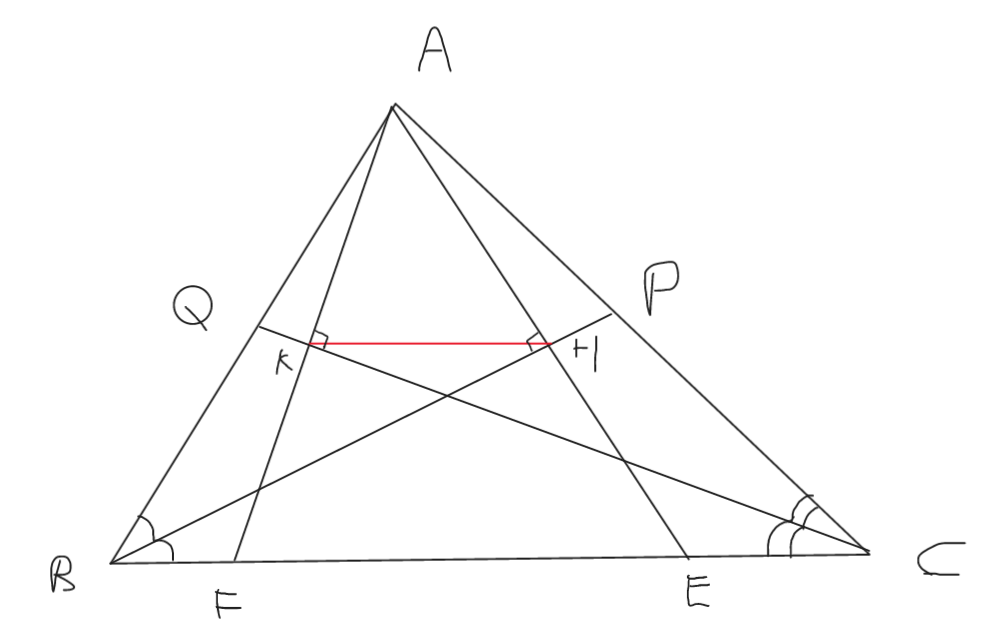
\includegraphics[width=3in, height=2in]{Screenshot_20230217_072116.png}}\\\\
\end{document}
